\def\disciplina {Calculo A}
\def\turma {00000}
\def\semestre {2016.1}
\def\numerodealunos {63}
\documentclass{article}
\usepackage[utf8]{inputenc}
\usepackage[T1]{fontenc}
\usepackage{graphicx}
\usepackage{palatino}
\usepackage{subcaption}
\title{Relatório de Notas de \disciplina\\Semestre \semestre}
\author{Melissa Weber Mendonça}
\date{}
\begin{document}
\maketitle
\section*{Distribuição de Notas}

Abaixo, uma tabela contendo as notas de \disciplina\ dos alunos da Turma \turma\ no semestre de \semestre.

\begin{table}[!h]
\end{table}

As Figuras~\ref{fig:prova1}, \ref{fig:prova2} e \ref{fig:prova3} representam a distribuição das notas para os \numerodealunos\ alunos desta turma.

\begin{figure}[ht]
   \centering
   \begin{subfigure}[b]{0.3\textwidth}
      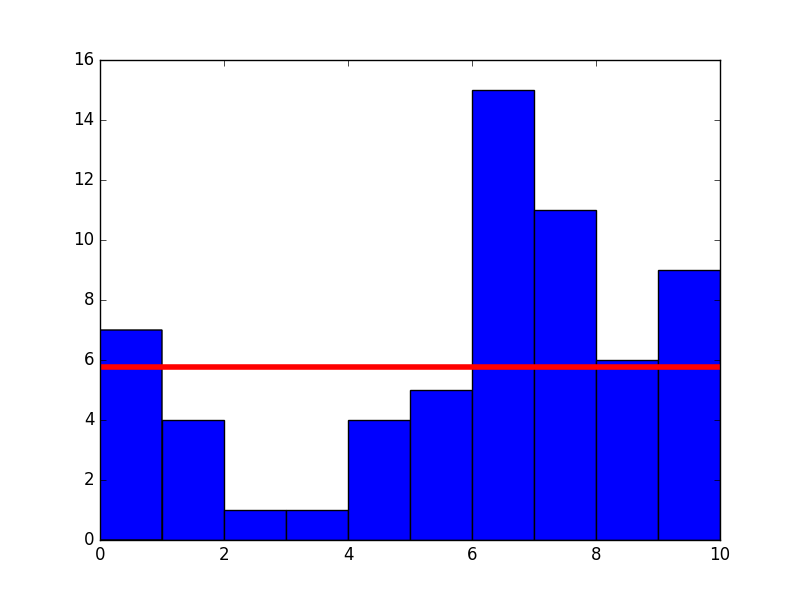
\includegraphics[width=4cm]{prova1.png}
      \caption{Notas da Prova 1.}
      \label{fig:prova1}
   \end{subfigure}
   ~
   \begin{subfigure}[b]{0.3\textwidth}
      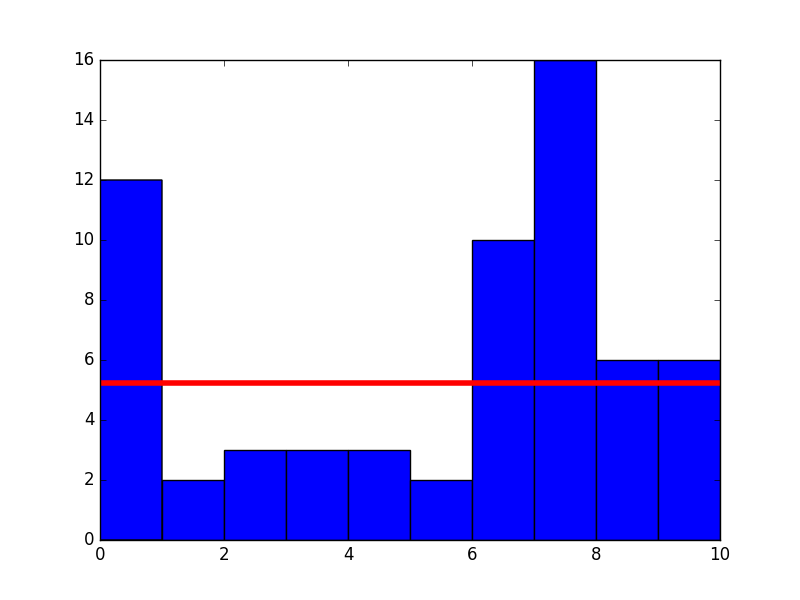
\includegraphics[width=4cm]{prova2.png}
      \caption{Notas da Prova 2.}
      \label{fig:prova2}
   \end{subfigure}
   ~
   \begin{subfigure}[b]{0.3\textwidth}
      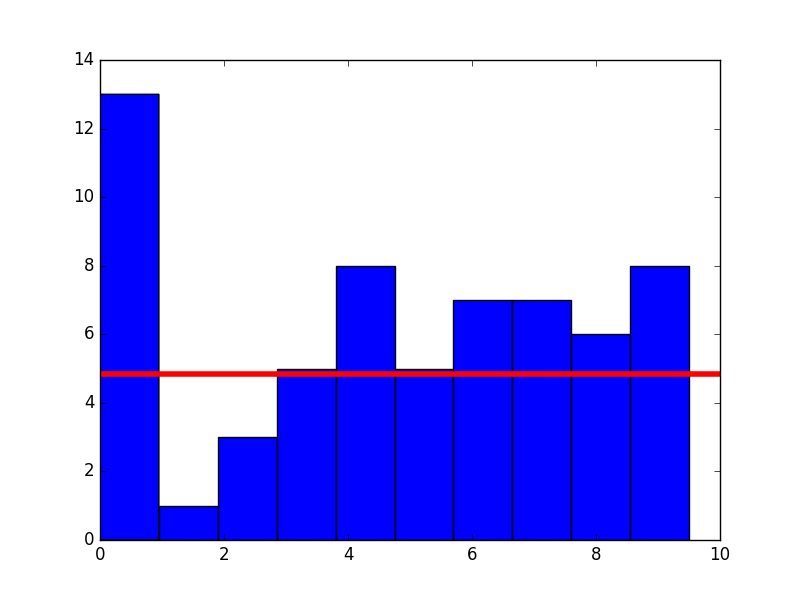
\includegraphics[width=4cm]{prova3.png}
      \caption{Notas da Prova 3.}
      \label{fig:prova3}
   \end{subfigure}
   \caption{Distrubuição de notas nas 3 provas.}
\end{figure}

\end{document}
